%% BioMed_Central_Tex_Template_v1.05
%%                                      %
%  bmc_article.tex            ver: 1.05 %
%                                       %

%%%%%%%%%%%%%%%%%%%%%%%%%%%%%%%%%%%%%%%%%%%%%%%%%%%%%%%%%%%%%%%%%%%%%
%%                                                                 %%	
%% For instructions on how to fill out this Tex template           %%
%% document please refer to Readme.pdf and the instructions for    %%
%% authors page on the biomed central website                      %%
%% http://www.biomedcentral.com/info/authors/                      %%
%%                                                                 %%
%% Please do not use \input{...} to include other tex files.       %%
%% Submit your LaTeX manuscript as one .tex document.              %%
%%                                                                 %%
%% All additional figures and files should be attached             %%
%% separately and not embedded in the \TeX\ document itself.       %%
%%                                                                 %%
%% BioMed Central currently use the MikTex distribution of         %%
%% TeX for Windows) of TeX and LaTeX.  This is available from      %%
%% http://www.miktex.org                                           %%
%%                                                                 %%
%%%%%%%%%%%%%%%%%%%%%%%%%%%%%%%%%%%%%%%%%%%%%%%%%%%%%%%%%%%%%%%%%%%%%


\NeedsTeXFormat{LaTeX2e}[1995/12/01]
\documentclass[10pt]{bmc_article}    

% Load packages
\usepackage{cite} % Make references as [1-4], not [1,2,3,4]
\usepackage{url}  % Formatting web addresses  
\usepackage{ifthen}  % Conditional 
\usepackage{multicol}   %Columns
\usepackage[utf8]{inputenc} %unicode support
%\usepackage[applemac]{inputenc} %applemac support if unicode package fails
%\usepackage[latin1]{inputenc} %UNIX support if unicode package fails
\urlstyle{rm} 
 
%%%%%%%%%%%%%%%%%%%%%%%%%%%%%%%%%%%%%%%%%%%%%%%%%	
%%                                             %%
%%  If you wish to display your graphics for   %%
%%  your own use using includegraphic or       %%
%%  includegraphics, then comment out the      %%
%%  following two lines of code.               %%   
%%  NB: These line *must* be included when     %%
%%  submitting to BMC.                         %% 
%%  All figure files must be submitted as      %%
%%  separate graphics through the BMC          %%
%%  submission process, not included in the    %% 
%%  submitted article.                         %% 
%%                                             %%
%%%%%%%%%%%%%%%%%%%%%%%%%%%%%%%%%%%%%%%%%%%%%%%%%               

%\def\includegraphic{}
%\def\includegraphics{}
\usepackage[]{graphicx}

\setlength{\topmargin}{0.0cm}
\setlength{\textheight}{21.5cm}
\setlength{\oddsidemargin}{0cm} 
\setlength{\textwidth}{16.5cm}
\setlength{\columnsep}{0.6cm}

\newboolean{publ}

%%%%%%%%%%%%%%%%%%%%%%%%%%%%%%%%%%%%%%%%%%%%%%%%%%
%%                                              %%
%% You may change the following style settings  %%
%% Should you wish to format your article       %%
%% in a publication style for printing out and  %%
%% sharing with colleagues, but ensure that     %%
%% before submitting to BMC that the style is   %%
%% returned to the Review style setting.        %%
%%                                              %%
%%%%%%%%%%%%%%%%%%%%%%%%%%%%%%%%%%%%%%%%%%%%%%%%%%

%Review style settings
\newenvironment{bmcformat}{\begin{raggedright}\baselineskip20pt\sloppy\setboolean{publ}{false}}{\end{raggedright}\baselineskip20pt\sloppy}

%Publication style settings
%\newenvironment{bmcformat}{\fussy\setboolean{publ}{true}}{\fussy}

% Begin ...
\begin{document}
\begin{bmcformat}

\title{Influenza peptide motif usage is most similar to that of the host
  organism it infects}
 
%%%%%%%%%%%%%%%%%%%%%%%%%%%%%%%%%%%%%%%%%%%%%%
%%                                          %%
%% Enter the authors here                   %%
%%                                          %%
%% Ensure \and is entered between all but   %%
%% the last two authors. This will be       %%
%% replaced by a comma in the final article %%
%%                                          %%
%% Ensure there are no trailing spaces at   %% 
%% the ends of the lines                    %%     	
%%                                          %%
%%%%%%%%%%%%%%%%%%%%%%%%%%%%%%%%%%%%%%%%%%%%%%

\author{Perry Evans\correspondingauthor$^{1,2}$%
       \email{samesense@gmail.com\correspondingauthor - charles@londonzoo.co.uk}%
      \and
         Will Dampier\correspondingauthor$^2$%
         \email{Jane E Doe\correspondingauthor - jane.e.doe@cambridge.co.uk}
          \and
         Yichuan Liu\correspondingauthor$^2$%
         \email{Jane E Doe\correspondingauthor - jane.e.doe@cambridge.co.uk}
          \and
         Lyle Ungar\correspondingauthor$^2$%
         \email{Jane E Doe\correspondingauthor - jane.e.doe@cambridge.co.uk}
       and 
         Aydin Tozeren$^3$%
         \email{John RS Smith - john.RS.Smith@cambridge.co.uk}%
      }
      
%%%%%%%%%%%%%%%%%%%%%%%%%%%%%%%%%%%%%%%%%%%%%%
%%                                          %%
%% Enter the authors' addresses here        %%
%%                                          %%
%%%%%%%%%%%%%%%%%%%%%%%%%%%%%%%%%%%%%%%%%%%%%%

\address{%
    \iid(1)Life Sciences Department, Kings College London, Cornwall House,%
        Waterloo Road, London, UK\\
    \iid(2)Department of Zoology, Cambridge, Waterloo Road, London, UK\\
    \iid(3)Marine Ecology Department, Institute of Marine Sciences Kiel, %
        D\"{u}sternbrooker Weg 20, 24105 Kiel, Germany
}%

\maketitle

%%%%%%%%%%%%%%%%%%%%%%%%%%%%%%%%%%%%%%%%%%%%%%
%%                                          %%
%% The Abstract begins here                 %%
%%                                          %%
%% The Section headings here are those for  %%
%% a Research article submitted to a        %%
%% BMC-Series journal.                      %%  
%%                                          %%
%% If your article is not of this type,     %%
%% then refer to the Instructions for       %%
%% authors on http://www.biomedcentral.com  %%
%% and change the section headings          %%
%% accordingly.                             %%   
%%                                          %%
%%%%%%%%%%%%%%%%%%%%%%%%%%%%%%%%%%%%%%%%%%%%%%

\begin{abstract}
        % Do not use inserted blank lines (ie \\) until main body of text.
        \paragraph*{Background:} Virus proteins harbor host peptide motifs that enable them to carry out necessary steps in their life-cycles by interacting with host proteins. The influenza virus infects many hosts, and its nucleotide sequence has been shown to evolve differently based on the host it infects. Here we examine differential peptide motif usage across groups of influenza virus sequences that are taken from the same host, and test the hypothesis that peptide motif usage for a virus group will be most similar to that of its host.
      
        \paragraph*{Results:} We annotate virus and host protein sequences with 153 confirmed peptide motifs, and cluster sequences matching motifs based on edit distance. For each host or virus group, we find distributions of cluster usage. We take the Jensen-Shannon divergence between distributions for hosts and influenza groups, and find that each influenza group matches best with its correct host.

        \paragraph*{Conclusions:} Peptide motif usage differs between hosts and between viruses derived from different hosts. Virus motif usage is most similar to the host from which it was taken. Phylogenetic distances are encoded in interactomes. http://bioinformatics.oxfordjournals.org/cgi/content/short/24/22/2579?rss=1

        \paragraph*{Availability:} Source code and paper, including all revisions, are accessible at http://github.com/JudoWill/flELM.
        
\end{abstract}

\ifthenelse{\boolean{publ}}{\begin{multicols}{2}}{}

%%%%%%%%%%%%%%%%%%%%%%%%%%%%%%%%%%%%%%%%%%%%%%
%%                                          %%
%% The Main Body begins here                %%
%%                                          %%
%% The Section headings here are those for  %%
%% a Research article submitted to a        %%
%% BMC-Series journal.                      %%  
%%                                          %%
%% If your article is not of this type,     %%
%% then refer to the instructions for       %%
%% authors on:                              %%
%% http://www.biomedcentral.com/info/authors%%
%% and change the section headings          %%
%% accordingly.                             %% 
%%                                          %%
%% See the Results and Discussion section   %%
%% for details on how to create sub-sections%%
%%                                          %%
%% use \cite{...} to cite references        %%
%%  \cite{koon} and                         %%
%%  \cite{oreg,khar,zvai,xjon,schn,pond}    %%
%%  \nocite{smith,marg,hunn,advi,koha,mouse}%%
%%                                          %%
%%%%%%%%%%%%%%%%%%%%%%%%%%%%%%%%%%%%%%%%%%%%%%

%%%%%%%%%%%%%%%%
%% Background %%
%%
\section*{Background}
Influenza A virus has the ability to infect a number of host
organisms, including human, chicken, swine, and horse. Nucleotide
sequences of the 2009 H1N1 pandemic influenza have been shown to have
a subsitution bias that depends on the host organism in which it
resides \cite{solovyov2010host}. In this study we examine the
possibility of a peptide motif usage bias that correlates with host
organism.

Virus proteins use many host peptide motifs to interact with host
proteins to accomplish necessary steps in the viral life-cycle
\cite{kadaveru13viral}. Host motifs on HIV proteins have been used to
predict patient response to therapy and interations with host proteins
\cite{chan2009decoding}.

Peptide sequence usage has been used to profile prokaryotic proteomes,
and the distances between profiles accuratly recovers the known
prokaryotic phylogeny \cite{jun2010whole}.

Here we demonstrate that the usage of peptide motifs differs between
influenza groups and host organisms. We show that an influenza group's
peptide motif profile if closest that of its host.
 
%%%%%%%%%%%%%%%%%%%%%%%%%%%%
%% Results and Discussion %%
%%
\section*{Results and Discussion}
  \subsection*{ELM profiles differ between hosts}

  \subsection*{ELM profiles differ between influenza groups}

  \subsection*{ELM profiles recover host phylogeny}

%%%%%%%%%%%%%%%%%%%%%%
\section*{Conclusions}
Here we investigated influenza group peptide biases, and checked to
see if they corresponded with those of their hosts.
  
%%%%%%%%%%%%%%%%%%
\section*{Methods}

\subsection*{Sequence Data}
All protein sequences used in the study were downloaded from
NCBI. Host organisms in NCBI have different degrees of protein
coverage. To standardize host and influenza sequence comparisons, we
used ortholgs common to all host species. Roundup
\cite{deluca2006roundup} was used with default settings to determine
ortholog clusters for human, chimpanzee, mouse, rat, cow, dog, pig,
horse, chicken and zebra finch proteins. We desired clusters with one
protein from each species. When one species had more than one protein
in an ortholog cluster, we picked one of these based on protein
length. The proteinn whose length was closest to the average length of
proteins from the other species was chosen.

NCBI influenza protein sequences are tagged with the host organism
they were taken from. For this study, we used influenza A sequences
taken from human, equine, swine, chicken, or duck. We further limited
influenza sequences by using only those that corresponded to proteins
hemagglutinin, neuraminidase, nucleocapsid protein, matrix protein 1,
matrix protein 2, nonstructural protein 1, nonstructural protein 2,
polymerase PB1, polymerase PA, polymerase PB2, or PB1-F2 protein. We
organized influenza sequences into groups based on the host organism
with which there were tagged and curation year.

All protein sequences were matched against regular expressions for 153
eukaryotic linear motifs cataloged in the ELM resource
\cite{gould2010elm}. Rapid matching was facilitated using cloud
computing provided by PiCloud. The host orgamisms had hits for all ELM
patterns, but the influenza sequences only had hits for XXX. The
sequences matched by the ELM patterns were not identical for host and
influenza. Most of the sequence matches on influenza were not present
on host orgamisms. Influenza and host sequences had few ELM sequence
hits in common. For these reasons, we reduced the twenty letter
alphabet to a four letter alphabet representing hydrophobic/small and
hydrophilic properties \cite{murphy2000simplified}. We converted host
ELM sequence hits to the simplified four letter alphabet, and used the
results as patterns for their respective ELMs. These simplified
patterns were then matched against the influenza protein sequences.

\subsection*{Phylogenies}
For each of the 153 ELMs, phylogenies were constructed from ELM
sequence hits using hierarchical clustering with average
linkage. Distances were found using Jensen-Shannon divergence for ELM
sequence distributions.

%%%%%%%%%%%%%%%%%%%%%%%%%%%%%%%%
\section*{Authors contributions}
    All authors contributed conceptually. Specific contributions are
    available at http://github.com/JudoWill/flELM/graphs/impact.

%%%%%%%%%%%%%%%%%%%%%%%%%%%
\section*{Acknowledgements}
  \ifthenelse{\boolean{publ}}{\small}{}
  This study was supported by the National Institutes of Health
  (NIH) grant number \# 232240 and by the National Science Foundation
  grant \# 235327. Additional support came from a Drexel University
  Calhoun Fellowship (WD) and from NIH training grant T32 HG000046
  (PE).
 
%%%%%%%%%%%%%%%%%%%%%%%%%%%%%%%%%%%%%%%%%%%%%%%%%%%%%%%%%%%%%
%%                  The Bibliography                       %%
%%                                                         %%              
%%  Bmc_article.bst  will be used to                       %%
%%  create a .BBL file for submission, which includes      %%
%%  XML structured for BMC.                                %%
%%                                                         %%
%%                                                         %%
%%  Note that the displayed Bibliography will not          %% 
%%  necessarily be rendered by Latex exactly as specified  %%
%%  in the online Instructions for Authors.                %% 
%%                                                         %%
%%%%%%%%%%%%%%%%%%%%%%%%%%%%%%%%%%%%%%%%%%%%%%%%%%%%%%%%%%%%%

%% {\ifthenelse{\boolean{publ}}{\footnotesize}{\small}
%%  \bibliographystyle{bmc_article}  % Style BST file
%%   \bibliography{refs} }     % Bibliography file (usually '*.bib' ) 
\bibliographystyle{bmc_article}  % Style BST file
  \bibliography{refs} 
%%%%%%%%%%%

\ifthenelse{\boolean{publ}}{\end{multicols}}{}

%%%%%%%%%%%%%%%%%%%%%%%%%%%%%%%%%%%
%%                               %%
%% Figures                       %%
%%                               %%
%% NB: this is for captions and  %%
%% Titles. All graphics must be  %%
%% submitted separately and NOT  %%
%% included in the Tex document  %%
%%                               %%
%%%%%%%%%%%%%%%%%%%%%%%%%%%%%%%%%%%

%%
%% Do not use \listoffigures as most will included as separate files

\section*{Figures}
  \subsection*{Figure 1 - Host ELM sequence usage}
      For each host, we show the distribution of ELM sequence counts.

      \begin{figure}
      \begin{center}
      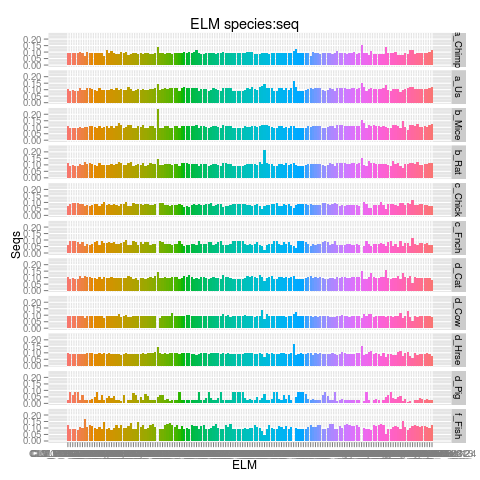
\includegraphics{figs/fig1}
      \end{center}
      \end{figure}

  \subsection*{Figure 2 - Influenza group LIG\_MAPK\_1 sequence usage}
     For each influenza group, we show the how many sequences match
     the pattern for the MAPK docking motif.

     \begin{figure}
      \begin{center}
      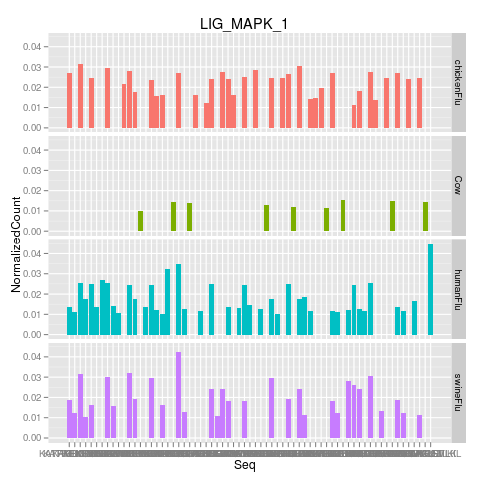
\includegraphics{figs/fig2}
      \end{center}
      \end{figure}

  \subsection*{Figure 3 - Host phylogeny}
     Using Jensen-Shannon divergence between (A) the distribution of
     ELM sequence hits or (B) clusters of ELM sequence hits produces
     the correct phylogeny.

     \begin{figure}
      \begin{center}
      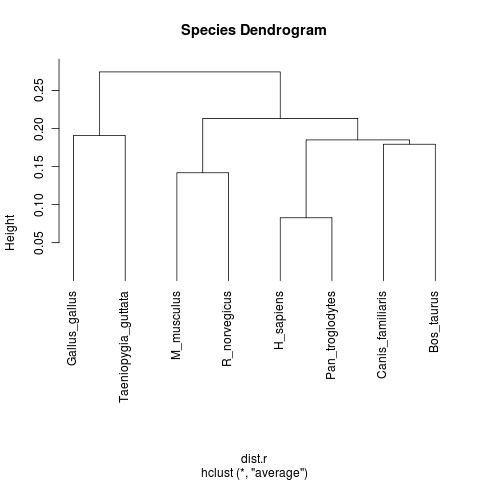
\includegraphics{figs/fig3}
      \end{center}
      \end{figure}  

%%%%%%%%%%%%%%%%%%%%%%%%%%%%%%%%%%%
%%                               %%
%% Tables                        %%
%%                               %%
%%%%%%%%%%%%%%%%%%%%%%%%%%%%%%%%%%%

%% Use of \listoftables is discouraged.
%%
\section*{Tables}
  \subsection*{Table 1 - Jensen-Shannon divergece between influenza groups and hosts}
    Here is an example of a \emph{small} table in \LaTeX\ using  
    \verb|\tabular{...}|. This is where the description of the table 
    should go. \par \mbox{}
    \par
    \mbox{
      \begin{tabular}{|c|c|c|}
        \hline \multicolumn{3}{|c|}{My Table}\\ \hline
        A1 & B2  & C3 \\ \hline
        A2 & ... & .. \\ \hline
        A3 & ..  & .  \\ \hline
      \end{tabular}
      }

%%%%%%%%%%%%%%%%%%%%%%%%%%%%%%%%%%%
%%                               %%
%% Additional Files              %%
%%                               %%
%%%%%%%%%%%%%%%%%%%%%%%%%%%%%%%%%%%

\section*{Additional Files}
  \subsection*{Additional file 1 --- Sample additional file title}
    Additional file descriptions text (including details of how to
    view the file, if it is in a non-standard format or the file extension).  This might
    refer to a multi-page table or a figure.

\end{bmcformat}
\end{document}







